\section{Desarrollo}

\subsection{Elección de Destinos}

Para realizar los experimentos se eligieron 3 universidades de distintos continentes para así poder presentar variedad en las rutas examinadas y poder analizar, luego, cuánto impactan los enlaces transatlánticos. En el Cuadro~\ref{tab:infouniv} se muestra la información de dichos destinos. Para el cálculo teórico del \textit{RTT}, las distancias se estimaron entre ciudad origen de los experimentos (\textsl{Ciudad Autónoma de Buenos Aires, Argentina}) y las respectivas ciudades de las universidades destino. Para ello se utilizó la herramienta de cálculo implementada en \textit{GeoBytes} \footnote{http://www.geobytes.com/citydistancetool.htm}. En la figura~\ref{fig:mapuniv1} se graficaron en un mapa los respectivos puntos con una estimación gráfica de la distancia lineal entre ellos.\\

\begin{table}[h]
    \centering
    \begin{tabular}{ | c | c | c | c | c |}
	    \hline
	    \textbf{Universidad} & \textbf{URL} & \textbf{IP} & \textbf{Continente} & \textbf{Distancia \textit{(km)}}\\ \hline
	    Univ. de California, Berkeley & http://www.berkeley.edu & 169.229.216.200 & América & 10412\\ \hline
	    Univ. de Oxford & http://www.ox.ac.uk & 163.1.60.42 & Europa & 11107\\ \hline
	    Universidad de Tokio & http://www.u-tokyo.ac.jp & 59.106.161.11 & Asia & 18372\\ \hline
    \end{tabular}
    \caption{Información sobre Universidades destino elegidas.}
    \label{tab:infouniv}
\end{table}

\begin{figure}[h!]
  \centering
  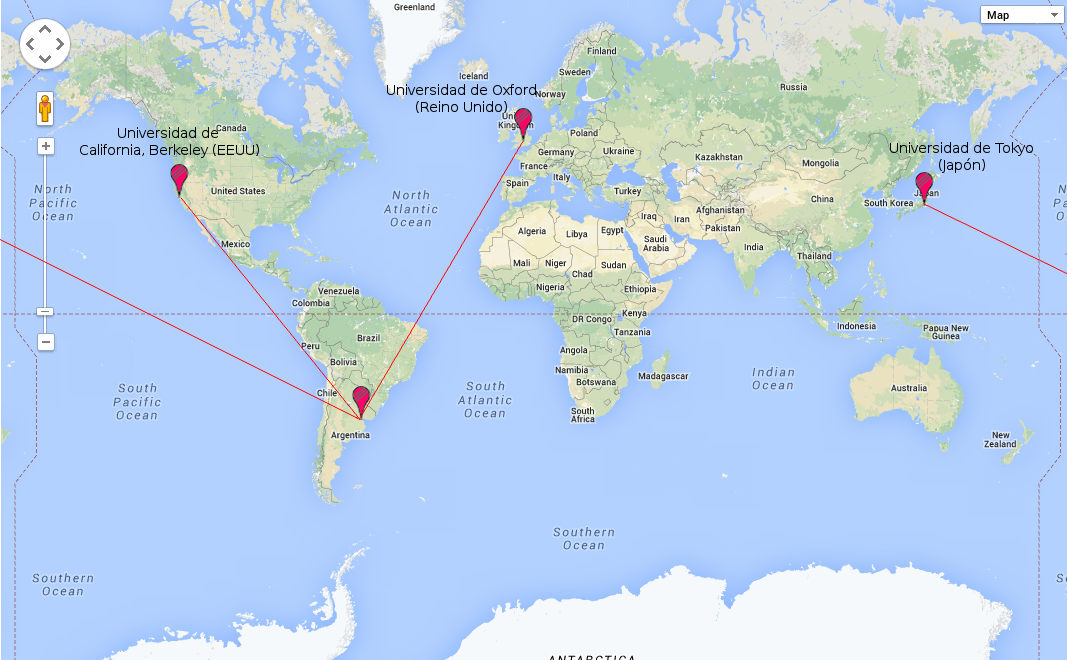
\includegraphics[width=0.7\textwidth]{./figs/map-univs1.png}
  \caption{Localización del origen y destinos con las respectivas distancias lineales aproximadas}
  \label{fig:mapuniv1}
\end{figure}

\subsection{Implementación de \textsl{Traceroute}}

El objetivo de la herramienta \textsl{traceroute} es examinar y trazar una porción de la ruta que atraviesa un paquete desde un origen hasta cierto destino a lo largo de las distintas redes por las que navega. Si bien tanto el sistema operativo Linux como la biblioteca de \textit{Python}, \textsl{Scapy}, proveen robustas implementaciones de esta utilidad, en principio no aplican para tomar tiempos, entre ellos el \textit{RTT}. Es por eso que se procedió a una implementación propia de \textsl{traceroute} basado en el enfoque de envío de paquetes \textit{ICMP}. En un \textit{ping} tradicional, dado un origen y un destino, el primero envía un paquete IP junto con un mensaje ICMP de tipo \textit{echo-request} a la espera de una respuesta satisfactoria de tipo \textit{echo-reply}. Para que esto suceda con éxito, el paquete ip debe tener un valor suficientemente grande en su campo \textit{ttl - time to live} de modo que los distintos nodos de la ruta lo reenvien hacia destino. En caso de que ese campo no sea suficiente para que el paquete llegue al destino deseado, el nodo que detecta el agotamiento de su \textit{ttl} responde con un mensaje ICMP de tipo {time-exceeded}. Tomando esta característica de la transmisión de paquetes y mensajes ICMP, la idea detrás de esta implementación de traceroute consiste en realizar sucesivos envíos de un paquete IP + mensaje ICMP \textit{echo-request} a destino comenzando con un \textit{ttl} unitario e incrementándolo en uno. De esta manera, el paquete 'muere' en distintos puntos del tramo y se puede identificar algunos de los nodos que se atraviesan ya que estos proveen su información al responder \textit{time-exceeded}.\\
\indent En el siguiente pseudocódigo se exhibe la idea detrás del algoritmo implementado.\\

\begin{algorithm}
\caption{traceroute (\textbf{in} $ipDest$, \textbf{in} $max\_hops$)}
\begin{algorithmic}[1]

\STATE $ttl \leftarrow 1$
\WHILE{$ttl < max\_hops$ y no se llego a destino}
	\STATE enviar mensaje ICMP \textsl{echo-request} sobre paquete IP con $ipDest$ y $ttl$
	\IF{hubo $respuesta$}
		\IF{$respuesta$ es de tipo \textsl{echo-reply}}
			\STATE imprimir datos de emisor de $respuesta$ y terminar
		\ELSE
			\STATE imprimir datos de emisor de $respuesta$
		\ENDIF
	\ENDIF
	\STATE $ttl \leftarrow ttl + 1$
\ENDWHILE
\end{algorithmic}
\end{algorithm}

\indent Al poder acceder al interior de este algoritmo, la modificación que se realizó fue la de realizar una diferencia de tiempo entre el instante previo al envío del mensaje y el instante posterior a la recepción de la respuesta. De esta manera, por cada paso de la ruta tenemos un valor empírico del $RTT$. Así podemos contar con todos los $round-trip$ $time$ de origen a cada nodo de la ruta y en particular a la de destino. En cierta forma esta versión de traceroute lleva implícita la funcionalidad de \textsl{ping}. Es importante notar que pueden existir valores de $ttl$ para los cuales no se obtenga respuesta (se supera el timeout del envío). Esto se puede deber a múltiples factores, pero no afecta la performance del algoritmo ya que se sigue adelante con un tiempo de vida mayor.\\

\subsection{Estimación de \textsl{RTT} empírico}

Basta con realizar un simple $ping$ a algún destino para notar a simple vista que los $round-trip$ $times$ empíricos son muy variables. Con el objetivo de obtener un valor algo más uniforme y representativo, exento de las particularidades temporales y espaciales de cada medición puntual, confeccionamos scripts para realizar $n$ mediciones de traceroute y poder volcar estos resultados en una matriz de datos. Por un lado, el script $rtt_traceroute$ de python toma un valor límite de $rtt$, una cantidad de iteraciones $n$ y un archivo de entrada con ternas de nombre, dns e ip de destino. Luego procede a ejecutar, para cada línea, $n$ iteraciones de traceroute, guardando el $rtt$ devuelto para el nodo final -destinatario- de la ruta. Por otro lado, el script en $Ruby$ lleva a cabo una tarea similar sólo que se vale de la herramienta 'traceroute' de Linux, la cual envía tres mensajes ICMP por valor de $ttl$, lo que totaliza 3 $rtt$ por cada ejecución. Finalmente, para procesar estos datos se crearon scripts de $Octave$ mediante los cuales se pudiera importar las matrices de resultados y realizar un promedio de los $round-trip$ $time$ para luego graficarlos en los diversos resultados presentados. Dependiendo de los experimentos la metodología puede haber variado un poco, caso en el cual se ampliará en la sección de Análisis.

\subsection{Detección de Enlaces Transatlánticos}

Con el fin de identificar posibles enlaces transatlánticos se creó el programa $trans\_atlantic\_traceroute$ en $Python$ que, dada la ruta con sus respectivos $rtt$ calculada por el algoritmo anterior, aplica la heurística recomendada en la consigna del trabajo para separar los posibles hops involucrados en un enlace del tipo buscado.

